% Author: Dr. Matthias Jung, DL9MJ
% Year: 2020
% TD431
\documentclass[convert = false, varwidth]{standalone}
\input{../common/settings.tex}
\usepackage{tikz,pgfplots}
\usetikzlibrary{arrows}

\usepackage{amsmath}
\usepackage{unicode-math}
\setmathfont{Fira Math}
\setmathfont[range=up]{Roboto}
\setmathfont[range=it]{Roboto-Italic}
\setmathfont[range=\int]{Fira Math}
\usepackage[euler]{textgreek}

\usepackage{filecontents}
\begin{filecontents*}{datafile.dat}
\end{filecontents*}

\pgfplotsset{compat=1.18}
\usepgfplotslibrary{fillbetween}

\begin{document}

\pgfplotsset{
  every axis plot/.append style={line width=0.8pt},
}

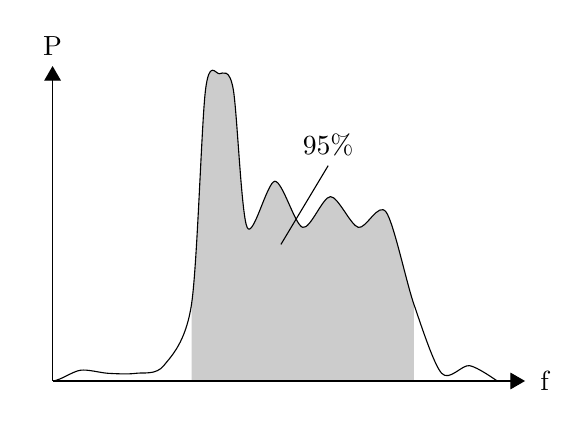
\begin{tikzpicture}
    \draw (0,4.25) node[]{P};
    \draw (6.25,0) node[]{f};

    %C:
    \draw (3.5,3.0) node[](A){95\%};
    \draw (A.south) -- ++(-0.6,-1.0);

    \begin{axis}[%
        /pgf/number format/1000 sep={ },
        /pgf/number format/use comma,        
        axis lines=middle,
        axis line style={-triangle 60},
        width=6cm,
        height=4cm,
        scale only axis,
        every major tick/.append style={thick, black},
        grid=major,
        grid style={line width=.1pt, draw=gray!10},
        major grid style={line width=.2pt,draw=gray!50},
        xticklabel=\empty,
        yticklabel=\empty,
        xtick style={draw=none},
        ytick style={draw=none},
        xmin=3,
        xmax=20,
        ymin=0.0,
        ymax=20.5,
        xmajorgrids=false,
        ymajorgrids=false,
        tick label style={font=\footnotesize}
    ]
    \addplot[color=black,name path=B] coordinates{
        (0,0)
        (1,0)
        (2,0)
        (3,0)
        (4,0)
        (5,0)
        (6,0)
        (7,0)
        (8,0)
        (8.5,0)
        (9,0)
        (9.5,0)
        (10,0)
        (11,0)
        (12,0)
        (13,0)
        (14,0)
        (15,0)
        (16,0)
        (17,0)
        (18,0)
        (19,0)
    };
    \addplot[color=black,smooth,name path=A] coordinates{
        (0,0)
        (1,0.5)
        (2,0.5)
        (3,0)
        (4,0.7)
        (5,0.5)
        (6,0.5)
        (7,1)
        (8,5)
        (8.5,18.9)
        (9,20.0)
        (9.5,19)
        (10,10)
        (11,13)
        (12,10)
        (13,12)
        (14,10)
        (15,11)
        (16,5)
        (17,0.5)
        (18,1.0)
        (19,0)
    };
    \addplot[gray, fill opacity=0.4] fill between[of=A and B,soft clip={domain=8:16}];

\end{axis}
\end{tikzpicture}%
\end{document}

